% Provenance (never printed): see sources/outline_sources.md (Year 3:
% sequence stratigraphy, accommodation and supply, systems tracts,
% cyclostratigraphy). Brief: sources/book5/BRIEFS.md, ch. 16. Curves from
% figdata/bachelor-3/shelf_model.py and lr04_periodogram.py. Exercise and
% problem values in the Book 5 scratch calculator calc/ch16.py. The Varden
% basin, its shelf and its core are invented.
\chapter{Estratigrafia de sequências}\label{ch:b3:sequence-stratigraphy}

Ao longo de uma seção sísmica de uma margem continental, os refletores se sobrepõem aos mais antigos,
depois avançam em direção à bacia, depois recuam em direção ao continente, e
o padrão se repete mais acima. Cada pacote registra uma disputa entre
duas taxas: a taxa com que se cria espaço para sedimento, por subsidência e pela
elevação do mar, e a taxa com que os rios o preenchem. A estratigrafia de sequências
lê a disputa a partir da geometria das camadas, e a
\omterm{def:b3:sequence-stratigraphy:cyclo}{cicloestratigrafia} lê o seu relógio a partir da espessura delas.

\begin{recall}
Acomodação, eustasia, nível relativo do mar, subsidência e a
bacia sedimentar estão no volume do primeiro ano, no capítulo sobre diagênese e bacias
sedimentares. A transgressão e a regressão marinhas e o ciclo do nível do mar de primeira
ordem estão no volume do segundo ano, no capítulo sobre a Terra fanerozoica; os
parâmetros de Milankovitch e a precessão climática, no capítulo sobre forçamento orbital
e as eras glaciais; o modelo de idade, no capítulo sobre arquivos climáticos
e indicadores. \omterm{def:b3:exploration-seismology:terminations}{Onlap}, \omterm{def:b3:exploration-seismology:terminations}{downlap}, \omterm{def:b3:exploration-seismology:terminations}{toplap}, \omterm{def:b3:exploration-seismology:terminations}{truncamento erosivo} e \omterm{def:b3:exploration-seismology:seismic-stratigraphy}{estratigrafia sísmica}
estão no Capítulo~\ref{ch:b3:exploration-seismology}. As séries de Fourier
e a transformada de Fourier estão nos livros de matemática.
\end{recall}

\section{Acomodação, suprimento e a linha de costa}\label{sec:b3:sequence-stratigraphy:shoreline}

Em qualquer ponto de uma bacia, o nível relativo do mar sobe à taxa $A = \dot E
+ \sigma$, a taxa eustática somada à taxa de subsidência (há queda quando $A < 0$).
O nível relativo do mar em um lugar é definido pelo nível global do mar e por
tudo o que move o terreno sob ele: a \omterm{def:b3:lithosphere-thermal-models:thermal-subsidence}{subsidência térmica}, a carga do
sedimento e a flexura que ela causa, a \omterm{def:b3:deformation-mechanisms:recrystallisation}{recuperação} isostática da crosta depois que um manto de gelo
derrete, e o empurrão lento do manto sob a placa. Um nível relativo do mar em elevação
cria acomodação, e o sedimento a preenche. Se a
linha de costa se desloca em direção ao mar ou em direção à terra depende de ambos, e não do nível do mar
sozinho.
% ledger: miller20:rsl

\begin{definition}[Regressão normal e regressão forçada]\label{def:b3:sequence-stratigraphy:regression}
Uma \emph{regressão normal}\index{regressão normal} é um deslocamento da linha de costa em direção ao mar
enquanto o nível relativo do mar sobe: o suprimento supera a
acomodação criada na linha de costa. Uma \emph{regressão forçada}\index{regressão forçada}
é um deslocamento em direção ao mar provocado por uma queda do nível relativo do mar: a
linha de costa é empurrada em direção à bacia independentemente do suprimento, e a terra deixada para trás
fica exposta e é erodida.
\end{definition}

\begin{definition}[Trajetória da linha de costa]\label{def:b3:sequence-stratigraphy:trajectory}
A \emph{trajetória da linha de costa}\index{trajetória da linha de costa} é o caminho da
linha de costa ao longo do tempo, desenhado em uma seção de mergulho no referencial do
sedimento, de modo que mostre tanto o deslocamento horizontal da linha de costa e a sua
subida ou descida em relação às camadas inferiores.
\end{definition}

Um perfil simples torna a disputa exata. Atrás da linha de costa, um topo plano
de largura $W$ fica ao nível do mar; à frente dele, uma frente de progradação de inclinação
$\tan\theta$ desce até o fundo da bacia, a uma altura $D$ abaixo. O suprimento de sedimento
$Q$ é um volume por unidade de tempo e por metro de costa (uma área por unidade de tempo
na seção).

\begin{proposition}[Trajetória da linha de costa]\label{prop:b3:sequence-stratigraphy:trajectory}
Se o nível relativo do mar sobe ($A \ge 0$) e o topo plano agradaciona uniformemente,
a linha de costa se move com
\[
\frac{\mathrm dx_s}{\mathrm dt} = \frac{Q - AW}{D};
\]
ela progradaciona enquanto $Q > AW$ e retrograda quando $AW > Q$. Se o nível relativo do mar
cai ($A < 0$), o topo plano não recebe nada e
\[
\frac{\mathrm dx_s}{\mathrm dt} = \frac{Q}{D} + \frac{|A|}{\tan\theta}.
\]
Nos dois casos, a trajetória sobe ou desce segundo o ângulo cuja tangente é
$A/(\mathrm dx_s/\mathrm dt)$.
\end{proposition}

\begin{proof}
Em um tempo $\mathrm dt$, o topo plano precisa de $AW\,\mathrm dt$ de sedimento para permanecer
ao nível do mar. O que sobra, $(Q - AW)\,\mathrm dt$, é espalhado na frente de progradação,
uma parede de altura $D$, que avança $(Q - AW)\,\mathrm dt/D$; um resto negativo
significa que o mar inunda o topo plano mais depressa do que ele se preenche. Quando o mar
desce, o topo plano fica acima da água e não recebe nada, e a linha de costa
desliza para baixo da antiga frente de progradação por $|A|\,\mathrm dt/\tan\theta$ sem nenhum
sedimento, enquanto todo o suprimento constrói a frente de progradação para a frente por $Q\,\mathrm
dt/D$. A linha de costa sobe $A\,\mathrm dt$ em relação às camadas inferiores
enquanto se desloca $\mathrm dx_s$, o que dá o ângulo.
\end{proof}

Uma \omterm{def:b3:sequence-stratigraphy:regression}{regressão normal}, portanto, exige um suprimento maior que a acomodação
criada no topo plano, e a sua trajetória sobe; uma \omterm{def:b3:sequence-stratigraphy:regression}{regressão forçada} acontece
independentemente do suprimento, e a sua trajetória desce. A razão entre as duas taxas,
frequentemente escrita $A/S$, classifica os padrões: progradação quando $A/S < 1$ no
topo plano, agradação próxima de 1, retrogradação acima disso. A mesma curva do nível do mar
pode, portanto, produzir uma regressão em uma margem rica em sedimento e uma
transgressão em uma margem pobre.

\section{Geometria estratal: sequências e tratos de sistemas}\label{sec:b3:sequence-stratigraphy:sequences}

As terminações de refletores do Capítulo~\ref{ch:b3:exploration-seismology}
são o vocabulário do método: \omterm{def:b3:exploration-seismology:terminations}{onlap} e \omterm{def:b3:exploration-seismology:terminations}{downlap} marcam a base de um
pacote, \omterm{def:b3:exploration-seismology:terminations}{toplap} e \omterm{def:b3:exploration-seismology:terminations}{truncamento erosivo} marcam o seu topo. Lidas em uma seção de mergulho, elas
dividem uma margem em pacotes limitados por superfícies de não deposição ou
de erosão, cada uma registrando um ciclo do nível relativo do mar.

\begin{definition}[Sequência deposicional e limite de sequência]\label{def:b3:sequence-stratigraphy:sequence}
Uma \emph{sequência deposicional}\index{sequência deposicional} é uma sucessão
de estratos geneticamente relacionados, sem quebra maior no interior, limitada na base
e no topo por discordâncias ou pelas concordâncias que as prolongam em direção à
bacia. Sua superfície limitante é o \emph{limite de
sequência}\index{limite de sequência}: uma discordância cortada por exposição e
erosão na plataforma durante uma queda do nível relativo do mar, que passa, em direção à
bacia, a uma concordância correlativa.
\end{definition}

\begin{definition}[Trato de sistemas]\label{def:b3:sequence-stratigraphy:tract}
Um \emph{trato de sistemas}\index{trato de sistemas} é o conjunto de
sistemas deposicionais (rio, costa, plataforma, talude) que estiveram ativos juntos durante uma
parte de um ciclo do nível relativo do mar, reconhecido pela sua posição na
sequência, pelas suas superfícies limitantes e pelo seu padrão de empilhamento. Distinguem-se
quatro:
\begin{itemize}
\item o \emph{trato de sistemas de estágio de queda}\index{trato de sistemas de estágio de queda},
  construído por \omterm{def:b3:sequence-stratigraphy:regression}{regressão forçada} enquanto o nível relativo do mar cai:
  foresets em degraus descendentes, desligados da antiga plataforma;
\item o \emph{trato de sistemas de mar baixo}\index{trato de sistemas de mar baixo},
  construído por \omterm{def:b3:sequence-stratigraphy:regression}{regressão normal} assim que o nível relativo do mar volta a subir,
  na posição mais baixa da linha de costa: uma cunha em agradação e progradação;
\item o \emph{trato de sistemas transgressivo}\index{trato de sistemas transgressivo},
  construído enquanto a linha de costa recua em direção ao continente, com unidades
  em retrogradação que se sobrepõem em \omterm{def:b3:exploration-seismology:terminations}{onlap} à antiga plataforma;
\item o \emph{trato de sistemas de mar alto}\index{trato de sistemas de mar alto},
  construído por \omterm{def:b3:sequence-stratigraphy:regression}{regressão normal} no final da subida, quando o aporte volta a
  superar a acomodação: foresets que progradam e fazem \omterm{def:b3:exploration-seismology:terminations}{downlap} sobre os depósitos subjacentes.
\end{itemize}
\end{definition}

\begin{definition}[Superfície transgressiva e superfície de inundação máxima]\label{def:b3:sequence-stratigraphy:surfaces}
A \emph{superfície transgressiva}\index{superfície transgressiva} é a primeira
\omterm{def:b3:sequence-stratigraphy:parasequence}{superfície de inundação} significativa acima dos depósitos de mar baixo: ela marca a
virada da linha de costa, da regressão para a transgressão. A \emph{superfície de
inundação máxima}\index{superfície de inundação máxima} marca a posição mais
continental da linha de costa, a virada da transgressão para a regressão de mar alto; os
foresets de mar alto fazem \omterm{def:b3:exploration-seismology:terminations}{downlap} sobre ela.
\end{definition}

\begin{definition}[Seção condensada e vale inciso]\label{def:b3:sequence-stratigraphy:condensed}
Uma \emph{seção condensada}\index{seção condensada} é um intervalo fino
depositado muito lentamente longe da linha de costa enquanto o mar inunda a plataforma
e o sedimento fica retido perto da costa: alguns centímetros ou decímetros
de argila, fósseis, glauconita ou fosfato que podem registrar um longo intervalo de tempo. Um
\emph{vale inciso}\index{vale inciso} é um vale fluvial escavado na
plataforma exposta enquanto o nível relativo do mar cai, e preenchido durante o
mar baixo e a transgressão seguintes.
\end{definition}

\begin{omfigure}
\begin{tikzpicture}[font=\scriptsize, x=0.9cm, y=1.25cm, >=Stealth]
% older highstand deposits below the sequence boundary
\fill[black!10] (0,0) -- (14,0) -- (14,0.4) -- (10,0.6) -- (6,2.8) -- (0,3.0) -- cycle;
\draw[black!35] (1.5,2.0) .. controls (3.2,1.95) and (4.5,1.2) .. (8.5,0.45);
\draw[black!35] (3.5,2.93) .. controls (4.8,2.85) and (6,1.6) .. (10.5,0.42);
% falling-stage systems tract
\fill[red!25] (6.0,2.8) -- (7.4,2.25) -- (8.4,1.85) -- (9.4,1.35) -- (10.4,0.75) -- (10.6,0.58) -- (10,0.6) -- cycle;
\draw[red!60!black] (6.6,2.56) .. controls (7.0,2.4) and (7.5,1.95) .. (8.0,1.70);
\draw[red!60!black] (7.6,2.17) .. controls (8.0,2.0) and (8.5,1.45) .. (9.0,1.15);
\draw[red!60!black] (8.6,1.75) .. controls (9.0,1.55) and (9.5,0.9) .. (10.0,0.6);
% lowstand wedge
\fill[orange!40] (9.2,1.45) -- (10.4,1.5) -- (11.5,1.0) -- (12.6,0.6) -- (13.4,0.44) -- (10.6,0.58) -- (10.4,0.75) -- cycle;
% incised valley and its fill
\fill[orange!30] (2.9,2.9) .. controls (3.3,2.3) and (3.9,2.3) .. (4.3,2.86) -- cycle;
% transgressive systems tract
\fill[green!45!black!35] (11.5,1.0) -- (10.4,1.5) -- (9.2,1.45) -- (8.4,1.85) -- (7.4,2.25) -- (6.0,2.8) -- (1.0,2.97) -- (1.0,3.05) -- (6.0,2.95) -- (7.6,2.5) -- (9.4,1.75) -- (10.8,1.45) -- cycle;
% highstand systems tract
\fill[blue!22] (0,3.62) -- (7.5,3.42) -- (9.8,2.2) -- (11.2,1.22) -- (10.8,1.45) -- (9.4,1.75) -- (7.6,2.5) -- (6.0,2.95) -- (1.0,3.05) -- (0,3.07) -- cycle;
\draw[blue!60!black] (4.0,3.52) .. controls (5.0,3.45) and (5.8,3.1) .. (6.6,2.79);
\draw[blue!60!black] (5.6,3.47) .. controls (6.6,3.4) and (7.4,2.8) .. (8.2,2.26);
\draw[blue!60!black] (6.8,3.44) .. controls (7.8,3.35) and (8.8,2.4) .. (9.7,1.69);
% surfaces
\draw[red!70!black, very thick] (0,3.0) -- (2.9,2.9) .. controls (3.3,2.3) and (3.9,2.3) .. (4.3,2.86) -- (6.0,2.8) -- (7.4,2.25) -- (8.4,1.85) -- (9.2,1.45);
\draw[red!70!black, very thick, densely dashed] (9.2,1.45) -- (9.4,1.35) -- (10.4,0.75) -- (10.6,0.58) -- (14,0.4);
\draw[green!40!black, thick] (11.5,1.0) -- (10.4,1.5) -- (9.2,1.45);
\draw[blue!60!black, thick] (0,3.07) -- (1.0,3.05) -- (6.0,2.95) -- (7.6,2.5) -- (9.4,1.75) -- (10.8,1.45) -- (11.5,1.03) -- (12.6,0.63) -- (13.4,0.47) -- (14,0.43);
% labels
\node[blue!50!black] at (2.6,3.36) {mar alto (HST)};
\node[green!35!black, anchor=south] at (4.8,3.92) {transgressivo (TST)};
\draw[green!35!black] (4.8,3.92) -- (4.4,3.01);
\node[red!60!black, anchor=west] at (10.1,2.45) {estágio de queda (FSST)};
\draw[red!60!black] (10.1,2.45) -- (8.8,1.62);
\node[orange!60!black, anchor=west] at (12.2,1.55) {mar baixo (LST)};
\draw[orange!60!black] (12.2,1.55) -- (11.2,0.85);
\node[anchor=north, align=center] at (3.6,2.25) {vale\\ inciso};
\node[red!70!black, anchor=north] at (1.4,2.95) {SB};
\node[red!70!black, anchor=north] at (12.0,0.38) {concordância correlativa};
\node[blue!60!black, anchor=west] at (12.7,1.1) {MFS};
\draw[blue!60!black] (12.7,1.1) -- (12.1,0.82);
\node[green!40!black, anchor=west] at (11.6,2.0) {TS};
\draw[green!40!black] (11.6,2.0) -- (10.9,1.27);
\node[blue!60!black, anchor=south] at (13.4,0.58) {condensado};
\node[anchor=west, black!60] at (0.2,0.35) {depósitos mais antigos};
\draw[->] (11.2,3.9) -- (12.6,3.9) node[right] {em direção à bacia};
\end{tikzpicture}

\par\smallskip{\small Anatomia de uma \omterm{def:b3:sequence-stratigraphy:sequence}{sequência deposicional} em seção de mergulho
(esquemática, escala vertical muito exagerada). O \omterm{def:b3:sequence-stratigraphy:sequence}{limite de sequência} (SB, em vermelho)
é uma discordância na plataforma, com um \omterm{def:b3:sequence-stratigraphy:condensed}{vale inciso}, e uma concordância correlativa
na bacia (tracejada); aqui ele está desenhado acima dos depósitos de estágio de
queda. A \omterm{def:b3:sequence-stratigraphy:surfaces}{superfície transgressiva} (TS) recobre a cunha de mar baixo; a \omterm{def:b3:sequence-stratigraphy:surfaces}{superfície de
inundação máxima} (MFS) recobre o trato transgressivo delgado e passa, em direção à
bacia, a uma \omterm{def:b3:sequence-stratigraphy:condensed}{seção condensada}; os foresets de mar alto fazem \omterm{def:b3:exploration-seismology:terminations}{downlap} sobre ela.}\label{fig:b3:sequence-stratigraphy:anatomy}
\end{omfigure}

Onde exatamente o \omterm{def:b3:sequence-stratigraphy:sequence}{limite de sequência} corre na bacia é uma convenção, e
os autores divergem: alguns o desenham na base dos depósitos de estágio de queda, onde
a queda começa, outros no seu topo, onde ela termina, como na figura acima.
Na plataforma não há ambiguidade: o limite é a superfície de exposição e
erosão, e os depósitos acima dele são mais novos que a queda.

Lido de baixo para cima, num ponto da plataforma externa, uma sequência registra o
ciclo: foresets de mar alto, uma superfície de exposição, talvez um preenchimento de
vale, a \omterm{def:b3:sequence-stratigraphy:surfaces}{superfície transgressiva}, camadas em retrogradação, um intervalo condensado na
\omterm{def:b3:sequence-stratigraphy:surfaces}{superfície de inundação máxima} e, em seguida, novamente foresets de mar alto. A hierarquia dos
ciclos é definida por suas causas: a abertura e o fechamento de oceanos para o
ciclo de primeira ordem, mudanças no volume de gelo e na velocidade de expansão do
assoalho oceânico para os ciclos mais curtos, e tectônica local e aporte para todos
eles.

\section{Parassequências e padrões de empilhamento}\label{sec:b3:sequence-stratigraphy:parasequences}

Dentro de um \omterm{def:b3:sequence-stratigraphy:tract}{trato de sistemas}, os menores pacotes que um geólogo mapeia numa falésia ou num
perfil de poço são unidades de raseamento para cima, com alguns metros a algumas dezenas de metros
de espessura, cobertas por uma superfície onde a água mais profunda retorna de repente.

\begin{definition}[Parassequência e superfície de inundação]\label{def:b3:sequence-stratigraphy:parasequence}
Uma \emph{parassequência}\index{parassequência} é uma sucessão relativamente concordante
de camadas geneticamente relacionadas, limitada por superfícies de inundação, na qual
a água torna-se mais rasa para cima: numa costa dominada por ondas, a lama de offshore passa
para areias de antepraia inferior e superior e para a praia. Uma \emph{superfície de
inundação}\index{superfície de inundação} é uma superfície através da qual fácies de água mais profunda
recobrem abruptamente fácies mais rasas, com evidências de um aprofundamento súbito.
\end{definition}

Uma única \omterm{def:b3:sequence-stratigraphy:parasequence}{parassequência} torna-se mais grossa para cima, e seu perfil de raios gama, baixo em areia
e alto em argila, forma uma silhueta em funil que se estreita para cima. A maneira como as
\omterm{def:b3:sequence-stratigraphy:parasequence}{parassequências} de um trato se empilham umas sobre as outras indica a tendência da
linha de costa: cada uma construída mais em direção ao mar do que a anterior (progradacional),
sobre a anterior (agradacional) ou mais para o continente (retrogradacional). Um perfil através do empilhamento
mostra a tendência diretamente: cada \omterm{def:b3:sequence-stratigraphy:parasequence}{parassequência} termina em fácies mais grossas e mais rasas
do que a de baixo, iguais a ela, ou mais finas e mais profundas.
Os tratos de mar alto e de mar baixo empilham-se de forma progradacional ou agradacional,
e o transgressivo, de forma retrogradacional. O próximo capítulo lê esses perfis fácies
por fácies.

\begin{omfigure}
\begin{tikzpicture}[font=\scriptsize, x=1cm, y=1cm]
% three logs: each parasequence a coarsening-upward wedge (grain size to the right)
% progradational
\begin{scope}[xshift=0cm]
\fill[yellow!45!brown!35] (0,0) -- (0.5,0) -- (1.4,1.1) -- (0,1.1) -- cycle;
\fill[yellow!45!brown!35] (0,1.1) -- (0.5,1.1) -- (1.8,2.2) -- (0,2.2) -- cycle;
\fill[yellow!45!brown!35] (0,2.2) -- (0.5,2.2) -- (2.2,3.3) -- (0,3.3) -- cycle;
\draw (0,0) -- (0.5,0) -- (1.4,1.1) -- (0.5,1.1) -- (1.8,2.2) -- (0.5,2.2) -- (2.2,3.3) -- (0,3.3) -- cycle;
\node[anchor=north, align=center] at (1.1,-0.1) {progradacional\\ (linha de costa avança para o mar)};
\end{scope}
% aggradational
\begin{scope}[xshift=4.2cm]
\fill[yellow!45!brown!35] (0,0) -- (0.5,0) -- (1.8,1.1) -- (0,1.1) -- cycle;
\fill[yellow!45!brown!35] (0,1.1) -- (0.5,1.1) -- (1.8,2.2) -- (0,2.2) -- cycle;
\fill[yellow!45!brown!35] (0,2.2) -- (0.5,2.2) -- (1.8,3.3) -- (0,3.3) -- cycle;
\draw (0,0) -- (0.5,0) -- (1.8,1.1) -- (0.5,1.1) -- (1.8,2.2) -- (0.5,2.2) -- (1.8,3.3) -- (0,3.3) -- cycle;
\node[anchor=north, align=center] at (1.1,-0.1) {agradacional\\ (linha de costa permanece)};
\end{scope}
% retrogradational
\begin{scope}[xshift=8.4cm]
\fill[yellow!45!brown!35] (0,0) -- (0.5,0) -- (2.2,1.1) -- (0,1.1) -- cycle;
\fill[yellow!45!brown!35] (0,1.1) -- (0.5,1.1) -- (1.8,2.2) -- (0,2.2) -- cycle;
\fill[yellow!45!brown!35] (0,2.2) -- (0.5,2.2) -- (1.4,3.3) -- (0,3.3) -- cycle;
\draw (0,0) -- (0.5,0) -- (2.2,1.1) -- (0.5,1.1) -- (1.8,2.2) -- (0.5,2.2) -- (1.4,3.3) -- (0,3.3) -- cycle;
\node[anchor=north, align=center] at (1.1,-0.1) {retrogradacional\\ (linha de costa recua para o continente)};
\end{scope}
% flooding surfaces
\foreach \s in {0,4.2,8.4} {
  \draw[omDef, thick] (\s-0.15,1.1) -- (\s+2.5,1.1);
  \draw[omDef, thick] (\s-0.15,2.2) -- (\s+2.5,2.2);
  \node[omDef, anchor=west] at (\s+2.5,1.1) {SI};
  \node[omDef, anchor=west] at (\s+2.5,2.2) {SI};
}
% grain-size axis
\draw[->] (0,3.6) -- (2.3,3.6) node[right] {granulometria mais grossa};
\node[anchor=east] at (0,3.6) {lama};
\end{tikzpicture}

\par\smallskip{\small Três \omterm{def:b3:sequence-stratigraphy:parasequence}{parassequências} empilhadas de três formas, desenhadas como
perfis de granulometria (a largura para a direita indica granulação mais grossa). Cada \omterm{def:b3:sequence-stratigraphy:parasequence}{parassequência}
torna-se mais grossa para cima, da lama offshore à areia de antepraia, e termina em uma \omterm{def:b3:sequence-stratigraphy:parasequence}{superfície de
inundação} (SI); o topo de cada uma é mais grosso que o da de baixo quando o empilhamento
progradar, igual quando agradar, mais fino quando
retrogradar.}\label{fig:b3:sequence-stratigraphy:stacking}
\end{omfigure}

\begin{inthefield}[Parassequências em uma falésia de deserto]
\begin{minipage}[t]{0.52\linewidth}\vspace{0pt}
As Book Cliffs, no leste de Utah, expõem depósitos de linha de costa do Cretáceo Superior
por dezenas de quilômetros. No Membro Kenilworth, acompanhado ao longo das falésias
de Price a Hatch Mesa, geólogos mapearam depósitos de planície costeira, antepraia,
plataforma interna e \omterm{def:b3:sequence-stratigraphy:condensed}{vale inciso}, e nove \omterm{def:b3:sequence-stratigraphy:parasequence}{parassequências} de granulação crescente para cima,
dominadas por ondas a tempestades, com 7 a \qty{32}{m} de espessura. Em direção à bacia
cada uma se divide em até quatro conjuntos menores de camadas de granulação crescente para cima, de 2 a
\qty{18}{m} de espessura; algumas areias de antepraia repousam sobre uma base abrupta, que o
estudo interpreta como depósitos de mar baixo.
\end{minipage}\hfill
\begin{minipage}[t]{0.44\linewidth}\vspace{0pt}
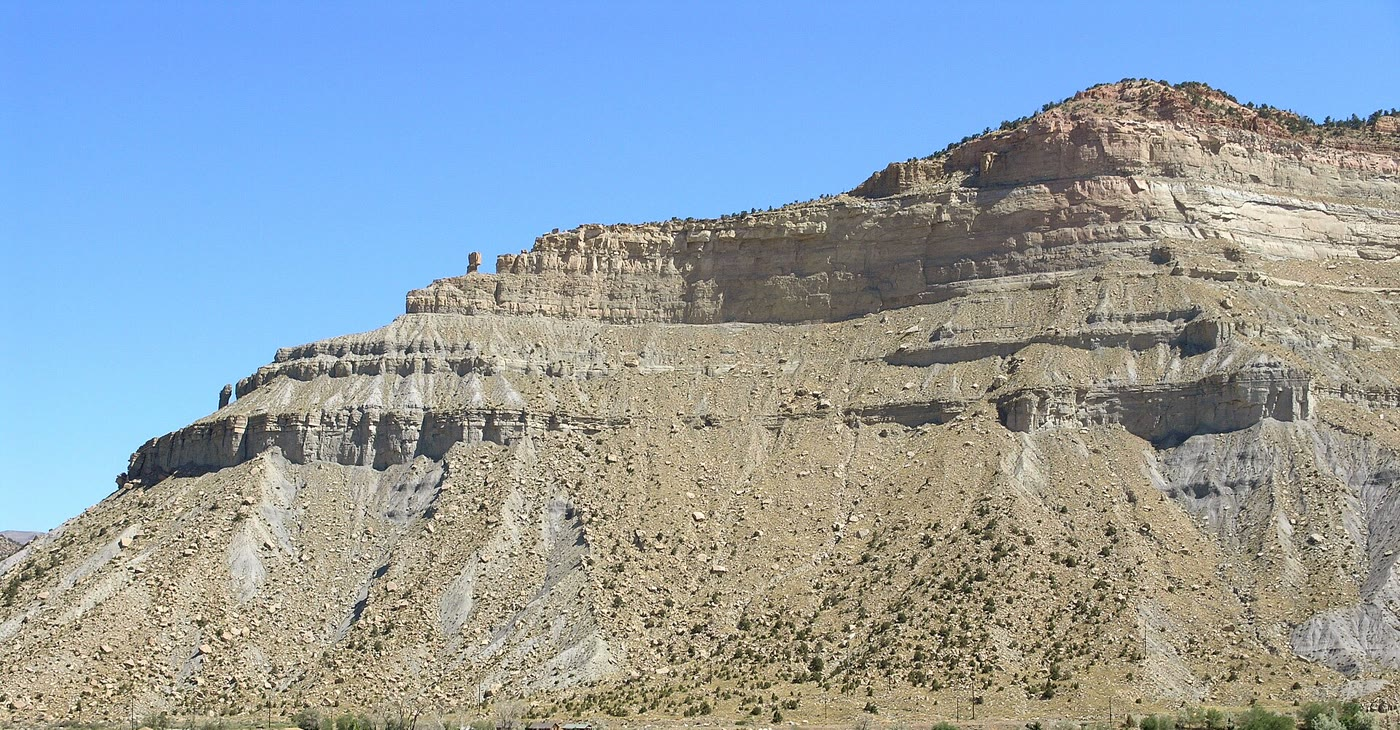
\includegraphics[width=\linewidth]{images/book5/b3-book-cliffs-helper.jpg}

{\scriptsize As Book Cliffs acima de Helper, Utah: cornijas de arenito claro se destacam
acima de encostas de lamito cinza. Foto de David Mackie, domínio público.}
\end{minipage}
\end{inthefield}
% ledger: pattison95:kenilworth, photo:b3-book-cliffs

\section{Um modelo direto de uma plataforma}\label{sec:b3:sequence-stratigraphy:model}

As regras das seções anteriores podem ser executadas como um modelo. A bacia Varden
é uma plataforma fictícia: uma rampa inclinada em direção à bacia a \qty{1.5}{m/km}, subsidindo
à taxa $\sigma = 0.02 + x/1200$ \unit{m/kyr} a uma distância $x$ (km) da charneira,
sob um nível do mar $E = -30\cos(2\pi t/400)$ (m, $t$ em kyr), alimentada por um rio que fornece
$Q = \qty{6000}{m^3/kyr}$ por metro de costa. A cada passo
de quinhentos anos, a bacia subside; o sedimento então preenche um \textit{topset} plano
até o nível do mar, onde a superfície antiga está submersa, e um
\textit{foreset} de declive 0.012 à sua frente, sendo a linha de costa posicionada de modo que o
volume acrescentado seja igual ao aporte; a terra exposta não recebe nada e, por
simplicidade, não sofre erosão. O modelo começa em mar baixo, após uma primeira
cunha construída com nível do mar constante.

\begin{omfigure}
\begin{tikzpicture}
\begin{groupplot}[group style={group size=1 by 2, vertical sep=0.35cm, x descriptions at=edge bottom},
  omrecord, width=0.86\linewidth, xmin=0, xmax=600,
  xtick={0,100,200,300,400,500,600},
  tick label style={font=\scriptsize}, label style={font=\small}]
\nextgroupplot[height=0.2\linewidth, ylabel={$E$ (m)}, ymin=-35, ymax=35,
  ytick={-30,0,30}]
\addplot[omDef, thick, domain=0:600, samples=121] {-30*cos(deg(2*pi*x/400))};
\nextgroupplot[height=0.3\linewidth, xlabel={tempo (kyr)}, ylabel={linha de costa $x_s$ (km)},
  ymin=0, ymax=60, ytick={0,20,40,60},
  scatter/classes={1={mark=*, red!70!black}, 2={mark=*, orange!80!black},
    3={mark=*, green!50!black}, 4={mark=*, blue!70!black}}]
% computed in figdata/bachelor-3/shelf_model.py
\addplot[scatter, only marks, mark size=0.9pt, scatter src=explicit symbolic]
  table[x=t, y=xs, meta=tract] {figdata/out/bachelor-3-shelf_model-shore.dat};
\node[font=\scriptsize, orange!60!black] at (axis cs:12,56) {TMB};
\node[font=\scriptsize, green!40!black] at (axis cs:70,40) {TT};
\node[font=\scriptsize, blue!60!black] at (axis cs:160,6) {TMA};
\node[font=\scriptsize, red!60!black] at (axis cs:300,22) {TEQ};
\node[font=\scriptsize, orange!60!black] at (axis cs:415,57) {TMB};
\node[font=\scriptsize, green!40!black] at (axis cs:520,45) {TT};
\node[font=\scriptsize, blue!60!black] at (axis cs:580,12) {TMA};
\end{groupplot}
\end{tikzpicture}

\par\smallskip{\small Acima, o nível eustático do mar do modelo de Varden;
abaixo, a posição da linha de costa, colorida por \omterm{def:b3:sequence-stratigraphy:tract}{trato de sistemas} (mar baixo
laranja, transgressivo verde, mar alto azul, estágio de queda vermelho), classificada
apenas a partir da saída do modelo: estágio de queda enquanto o nível relativo do mar cai
na linha de costa, transgressivo enquanto a linha de costa recua, mar baixo ou
mar alto enquanto ela avança sob um mar em elevação, após uma queda ou após uma
transgressão.}\label{fig:b3:sequence-stratigraphy:series}
\end{omfigure}

A figura acima acompanha a linha de costa ao longo do tempo, e a de baixo
mostra os depósitos que ela deixou. Os tratos aparecem sem nenhuma regra escrita no
modelo além do preenchimento e da subsidência. A cunha de mar baixo no início fica
bem afastada; a elevação do mar leva a linha de costa \qty{38}{km} para o continente na
primeira transgressão, e os \textit{foresets} de mar alto voltam a avançar à medida que a elevação desacelera.
Então a queda começa: a linha de costa é empurrada em direção à bacia em \qty{33}{km} em
\qty{187}{kyr}, deixando \textit{foresets} finos em degraus descendentes e uma plataforma exposta
atrás, o trato de estágio de queda. Seguem uma nova cunha de mar baixo, uma segunda transgressão
e um novo mar alto. A velocidade da \omterm{def:b3:sequence-stratigraphy:regression}{regressão forçada} no modelo
coincide com a fórmula da proposição dentro de poucos por cento; sob um mar em
elevação, o topset do modelo não se acumula uniformemente, já que a subsidência
cresce em direção à bacia, e a fórmula serve apenas como guia.

\begin{omfigure}
\begin{tikzpicture}
\begin{axis}[omsection, width=0.95\linewidth, height=0.42\linewidth,
  xmin=0, xmax=70, ymin=-150, ymax=40, clip=true,
  xlabel={distância em direção à bacia (km)}, ylabel={elevação atual (m)},
  xtick={0,10,20,30,40,50,60,70}, ytick={-150,-100,-50,0},
  tick label style={font=\scriptsize}, label style={font=\small}]
% computed in figdata/bachelor-3/shelf_model.py
\addplot[fill=black!10, draw=none] table[x=x, y=z0] {figdata/out/bachelor-3-shelf_model-surfaces.dat} -- (axis cs:120,-300) -- (axis cs:0,-300) -- cycle;
\addplot[fill=orange!45, draw=none] table[x=x, y=z] {figdata/out/bachelor-3-shelf_model-poly1.dat};
\addplot[fill=green!45!black!35, draw=none] table[x=x, y=z] {figdata/out/bachelor-3-shelf_model-poly2.dat};
\addplot[fill=blue!25, draw=none] table[x=x, y=z] {figdata/out/bachelor-3-shelf_model-poly3.dat};
\addplot[fill=red!30, draw=none] table[x=x, y=z] {figdata/out/bachelor-3-shelf_model-poly4.dat};
\addplot[fill=orange!45, draw=none] table[x=x, y=z] {figdata/out/bachelor-3-shelf_model-poly5.dat};
\addplot[fill=green!45!black!35, draw=none] table[x=x, y=z] {figdata/out/bachelor-3-shelf_model-poly6.dat};
\addplot[fill=blue!25, draw=none] table[x=x, y=z] {figdata/out/bachelor-3-shelf_model-poly7.dat};
\addplot[black!45, very thin] table[x=x, y=z40] {figdata/out/bachelor-3-shelf_model-surfaces.dat};
\addplot[black!45, very thin] table[x=x, y=z80] {figdata/out/bachelor-3-shelf_model-surfaces.dat};
\addplot[black!45, very thin] table[x=x, y=z120] {figdata/out/bachelor-3-shelf_model-surfaces.dat};
\addplot[black!45, very thin] table[x=x, y=z160] {figdata/out/bachelor-3-shelf_model-surfaces.dat};
\addplot[black!45, very thin] table[x=x, y=z240] {figdata/out/bachelor-3-shelf_model-surfaces.dat};
\addplot[black!45, very thin] table[x=x, y=z280] {figdata/out/bachelor-3-shelf_model-surfaces.dat};
\addplot[black!45, very thin] table[x=x, y=z320] {figdata/out/bachelor-3-shelf_model-surfaces.dat};
\addplot[black!45, very thin] table[x=x, y=z360] {figdata/out/bachelor-3-shelf_model-surfaces.dat};
\addplot[black!45, very thin] table[x=x, y=z440] {figdata/out/bachelor-3-shelf_model-surfaces.dat};
\addplot[black!45, very thin] table[x=x, y=z480] {figdata/out/bachelor-3-shelf_model-surfaces.dat};
\addplot[black!45, very thin] table[x=x, y=z520] {figdata/out/bachelor-3-shelf_model-surfaces.dat};
\addplot[black!45, very thin] table[x=x, y=z560] {figdata/out/bachelor-3-shelf_model-surfaces.dat};
\addplot[black, thin] table[x=x, y=z600] {figdata/out/bachelor-3-shelf_model-surfaces.dat};
\addplot[black, only marks, mark=*, mark size=0.5pt] table[x=xs, y=zfinal] {figdata/out/bachelor-3-shelf_model-shore.dat};
\node[font=\scriptsize, blue!50!black] at (axis cs:6,4) {TMA};
\node[font=\scriptsize, green!30!black] at (axis cs:12,-22) {TT};
\node[font=\scriptsize, red!60!black] at (axis cs:35,-25) {TEQ};
\node[font=\scriptsize, orange!60!black] at (axis cs:57.5,-60) {TMB};
\node[font=\scriptsize, green!30!black] at (axis cs:36,2) {TT};
\node[font=\scriptsize, blue!50!black] at (axis cs:8,26) {TMA};
\end{axis}
\end{tikzpicture}

\par\smallskip{\small A plataforma de Varden após \qty{600}{kyr}, em sua posição atual
(escala vertical exagerada cerca de 170 vezes). As cores são os
\omterm{def:b3:sequence-stratigraphy:tract}{tratos de sistemas}: mar baixo laranja, transgressivo verde, mar alto azul,
estágio de queda vermelho; o cinza é a rampa mais antiga e a primeira cunha. As linhas finas são
o fundo do mar a cada \qty{40}{kyr}; os pontos pretos traçam a linha de costa a cada
\qty{2}{kyr}. Calculado pelo modelo direto do
texto.}\label{fig:b3:sequence-stratigraphy:section}
\end{omfigure}


O nível relativo do mar começa a cair na linha de costa alguns milhares de anos
após o alto eustático, porque a subsidência precisa primeiro ser superada,
e termina alguns milhares de anos antes do baixo eustático. A queda na
linha de costa dura assim menos da metade do ciclo eustático, e tanto mais quanto
mais rápido a bacia subsidir.

Modelos desse tipo são o teste honesto de uma interpretação, e também mostram
seus limites. A mesma seção pode ser construída por histórias diferentes: uma queda mais rápida
com menos suprimento, ou uma mais lenta com mais, ou uma mudança de subsidência
em vez do nível do mar, já que a geometria registra apenas o nível relativo do mar
e o suprimento. As cartas globais de ciclos do nível do mar, construídas a partir de margens nas
décadas de 1970 e 1980, fixaram a cronologia de muitas quedas que a perfuração desde então
confirmou em grande parte para trechos do Cretáceo Superior ao Mioceno, mas suas
amplitudes, como uma queda de \qty{160}{m} no Oligoceno médio, são altas demais
por um fator de 2 a 3. As amplitudes eustáticas são hoje obtidas a partir de
isótopos de oxigênio e de poços com backstripping, e as sequências de uma margem são
lidas primeiro como um registro local.
% ledger: miller20:epr, miller20:rsl

\section{Cicloestratigrafia}\label{sec:b3:sequence-stratigraphy:cyclo}

Muitas sucessões se repetem em intervalos regulares de espessura: pares de margas e calcários,
pacotes de cinco pares, conjuntos maiores de pacotes. Se a repetição
for ritmada pelos parâmetros de Milankovitch, a espessura dos
ciclos se converte em tempo.

\begin{definition}[Cicloestratigrafia e ajuste astronômico]\label{def:b3:sequence-stratigraphy:cyclo}
A \emph{cicloestratigrafia}\index{cicloestratigrafia} identifica e mede
ciclos regulares em sucessões sedimentares e os interpreta como registros de
forçamento periódico, principalmente as variações da órbita e do eixo da Terra.
O \emph{ajuste astronômico}\index{ajuste astronômico} atribui idades a uma
sucessão ao casar seus ciclos, um a um, com uma série astronômica calculada
(excentricidade, obliquidade, precessão ou insolação), o que transforma os
ciclos em um modelo de idade.
\end{definition}

Os períodos calculados vêm da solução do movimento do Sistema Solar.
A excentricidade da órbita da Terra tem um termo principal de \qty{405}{kyr}, e
quatro termos próximos de \qty{100}{kyr} (95, 99, 124 e \qty{131}{kyr}); a
obliquidade tem um termo principal de \qty{41.0}{kyr}, com termos menores em 39.6 e
\qty{53.7}{kyr}. A precessão climática combina a precessão do eixo
com o movimento do periélio, nas frequências $p_0 + g_i$, em que $p_0 =
50.47''$ por ano e os $g_i$ são frequências das órbitas planetárias; seus
períodos principais são 23.7, 22.4, 19.1 e \qty{19.0}{kyr}. O termo de \qty{405}{kyr}
é o mais estável, e serve de metrônomo para sucessões mais antigas.
% ledger: la04:eccentricity, la04:obliquity, la04:precession

\begin{omfigure}
\begin{tikzpicture}
\begin{groupplot}[group style={group size=2 by 1, horizontal sep=0.5cm, y descriptions at=edge left},
  omrecord, width=0.52\linewidth, height=0.33\linewidth,
  xmin=0, xmax=0.06, ymin=0, ymax=1.18, clip=false,
  xtick={0,0.02,0.04,0.06}, xticklabels={0,0.02,0.04,0.06}, scaled x ticks=false,
  ytick={0,0.5,1}, title style={font=\small},
  tick label style={font=\scriptsize}, label style={font=\small},
  xlabel={frequência (ciclos por kyr)}]
\nextgroupplot[title={(a) 0 a \qty{1000}{ka}}, ylabel={potência relativa}]
\draw[black!40, densely dotted] (axis cs:0.01,0) -- (axis cs:0.01,1.05);
\draw[black!40, densely dotted] (axis cs:0.0244,0) -- (axis cs:0.0244,1.05);
\draw[black!40, densely dotted] (axis cs:0.0429,0) -- (axis cs:0.0429,1.05);
\draw[black!40, densely dotted] (axis cs:0.0526,0) -- (axis cs:0.0526,1.05);
\node[font=\scriptsize, anchor=south] at (axis cs:0.01,1.05) {100};
\node[font=\scriptsize, anchor=south] at (axis cs:0.0244,1.05) {41};
\node[font=\scriptsize, anchor=south] at (axis cs:0.0429,1.05) {23};
\node[font=\scriptsize, anchor=south] at (axis cs:0.0526,1.05) {19};
% computed in figdata/bachelor-3/lr04_periodogram.py
\addplot[omDef, thick] table[x=f, y=p] {figdata/out/bachelor-3-lr04_periodogram-young.dat};
\nextgroupplot[title={(b) 1250 a \qty{2500}{ka}}]
\draw[black!40, densely dotted] (axis cs:0.01,0) -- (axis cs:0.01,1.05);
\draw[black!40, densely dotted] (axis cs:0.0244,0) -- (axis cs:0.0244,1.05);
\draw[black!40, densely dotted] (axis cs:0.0429,0) -- (axis cs:0.0429,1.05);
\draw[black!40, densely dotted] (axis cs:0.0526,0) -- (axis cs:0.0526,1.05);
\node[font=\scriptsize, anchor=south] at (axis cs:0.01,1.05) {100};
\node[font=\scriptsize, anchor=south] at (axis cs:0.0244,1.05) {41};
\node[font=\scriptsize, anchor=south] at (axis cs:0.0429,1.05) {23};
\node[font=\scriptsize, anchor=south] at (axis cs:0.0526,1.05) {19};
\addplot[omDef, thick] table[x=f, y=p] {figdata/out/bachelor-3-lr04_periodogram-old.dat};
\end{groupplot}
\end{tikzpicture}

\par\smallskip{\small \omterm{def:b3:sequence-stratigraphy:periodogram}{Periodogramas} do empilhamento de isótopos de oxigênio bentônicos LR04
em duas janelas (sem tendência, janela de Hann, normalizados pelo maior pico);
as linhas pontilhadas marcam períodos de 100, 41, 23 e \qty{19}{kyr}. (a) No último
milhão de anos: a faixa de \qty{100}{kyr} domina. (b) De 2.5 a
\qty{1.25}{Ma}: a obliquidade de \qty{41}{kyr} domina.}\label{fig:b3:sequence-stratigraphy:periodogram}
\end{omfigure}
% ledger: data:lr04, lr04:tuning

\begin{definition}[Periodograma]\label{def:b3:sequence-stratigraphy:periodogram}
O \emph{periodograma}\index{periodograma} de uma série $y_0, \dots, y_{N-1}$
amostrada com passo $\Delta$ (no tempo ou na profundidade), após a remoção de sua média e
de sua tendência e da multiplicação por uma janela $w_k$, é
\[
P(f_j) = \Bigl|\sum_{k=0}^{N-1} w_k y_k\, e^{-2\pi i f_j k\Delta}\Bigr|^2,
\qquad f_j = \frac{j}{N\Delta},\ j = 1, \dots, \frac N2:
\]
a potência da série em cada frequência $f_j$, o quadrado do módulo de
sua transformada discreta de Fourier.
\end{definition}

Dois números delimitam o que um \omterm{def:b3:sequence-stratigraphy:periodogram}{periodograma} consegue enxergar. Seu passo de frequência, $1/(N\Delta)$,
o inverso do comprimento do registro, é a resolução: dois períodos cujas
frequências diferem em menos não podem ser separados. Sua frequência mais alta, a
frequência de Nyquist $1/(2\Delta)$, é atingida com duas amostras por ciclo; um
ciclo mais curto não se perde, mas é rebatido como um falso ciclo mais longo. A janela,
aqui uma janela de Hann, suaviza as extremidades da série para que um pico forte não
vaze potência por todo o espectro.


Os \omterm{def:b3:sequence-stratigraphy:periodogram}{periodogramas} acima são o caso trabalhado. No último milhão de anos, o pico mais forte
cai na faixa de \qty{100}{kyr} (em \qty{91}{kyr} na grade de frequências
de um registro de \qty{1000}{kyr}, cujos vizinhos são 100 e \qty{83}{kyr}),
a obliquidade tem um terço de sua potência e a precessão alguns por cento;
entre 2.5 e \qty{1.25}{Ma} a obliquidade domina o registro e a
faixa de \qty{100}{kyr} tem um sexto de sua potência. Há uma cautela embutida nos
dados: a escala de tempo do LR04 foi ela mesma obtida ajustando o empilhamento a um modelo simples
de gelo forçado pela insolação de verão a \ang{65}\,N, restringido por
taxas de sedimentação empilhadas para evitar sobreajuste, de modo que encontrar períodos orbitais nela
é em parte circular. O teste que não é circular é o feito em profundidade,
antes de qualquer ajuste: se as razões entre as espessuras dos ciclos coincidirem com as
razões entre os períodos orbitais, o forçamento fica demonstrado, e as espessuras fornecem
a taxa de sedimentação.
% ledger: lr04:tuning, la04:obliquity

\begin{method}[Taxa de sedimentação a partir da espessura dos ciclos]\label{met:b3:sequence-stratigraphy:cycles}
\begin{enumerate}
\item calcule o \omterm{def:b3:sequence-stratigraphy:periodogram}{periodograma} da série em profundidade, com sua resolução
  $1/L$ para uma seção de comprimento $L$ e seu limite de Nyquist $1/(2\Delta z)$;
\item liste os comprimentos de onda dos picos significativos, $\lambda = 1/f$;
\item compare suas razões com as dos períodos orbitais (405 : 100 : 41
  : 23, ou 21 para uma precessão média); a coincidência de três picos é um argumento forte,
  um pico isolado não é argumento algum;
\item divida cada comprimento de onda pelo seu período: os quocientes, que devem
  concordar, fornecem a taxa de sedimentação.
\end{enumerate}
\end{method}

Uma taxa de sedimentação obtida dessa forma é uma média sobre o ciclo e
supõe uma taxa constante: uma mudança de taxa dentro da seção alonga os
picos, e uma lacuna elimina ciclos sem aviso. Sucessões longas são, portanto,
ajustadas ciclo a ciclo contra a série calculada, começando pelo ciclo de \qty{405}{kyr}
e conferidas com idades radiométricas onde os leitos vulcânicos permitem.

\section{Exercícios}

\begin{exercise}[$\star$]\label{exo:b3:sequence-stratigraphy:1}
Em um ponto de uma plataforma, o nível do mar eustático sobe a \qty{0.5}{m/kyr} e
a bacia subside a \qty{0.1}{m/kyr}. Calcule a taxa de elevação relativa
do nível do mar e a acomodação criada em \qty{20}{kyr}. Qual é a
taxa relativa se, em vez disso, o mar descer a \qty{0.3}{m/kyr}?
\end{exercise}

\begin{exercise}[$\star$]\label{exo:b3:sequence-stratigraphy:2}
Para cada caso, nomeie o \omterm{def:b3:sequence-stratigraphy:tract}{trato de sistemas} que está sendo construído: (a) o nível relativo do mar
desce, a linha de costa avança em direção ao mar; (b) o nível relativo do mar sobe, a
linha de costa recua em direção ao continente; (c) o nível relativo do mar sobe lentamente no fim de um
ciclo, a linha de costa avança em direção ao mar e os \textit{foresets} fazem \omterm{def:b3:exploration-seismology:terminations}{downlap} sobre uma
\omterm{def:b3:sequence-stratigraphy:surfaces}{superfície de inundação máxima}; (d) o nível relativo do mar acaba de começar a subir após uma
queda, e a linha de costa ainda avança em direção ao mar.
\end{exercise}

\begin{exercise}[$\star$]\label{exo:b3:sequence-stratigraphy:3}
Um perfil de poço mostra três \omterm{def:b3:sequence-stratigraphy:parasequence}{parassequências}, cada uma com granulação crescente para cima. Os topos das
três, da inferior para a superior, são areia fina, areia média e areia grossa com
laminação de praia. Nomeie o padrão de empilhamento, o deslocamento da linha de costa e
os \omterm{def:b3:sequence-stratigraphy:tract}{tratos de sistemas} aos quais ele pode pertencer. O que significaria a ordem oposta?
\end{exercise}

\begin{exercise}[$\star$]\label{exo:b3:sequence-stratigraphy:4}
Uma falésia mostra pares de margas e calcários agrupados em conjuntos de cinco; um
conjunto tem \qty{1.6}{m} de espessura. Interprete os pares e os conjuntos com os
períodos orbitais e calcule a taxa de sedimentação a partir dos conjuntos.
\end{exercise}

\begin{exercise}[$\star\star$]\label{exo:b3:sequence-stratigraphy:5}
Uma plataforma tem um \textit{topset} com \qty{20}{km} de largura, um \textit{foreset} com \qty{50}{m} de altura e um
aporte de \qty{4000}{m^3/kyr} por metro de costa; o nível relativo do mar sobe
a \qty{0.15}{m/kyr}. Calcule a velocidade da linha de costa. Com que taxa de
subida ela ficaria parada?
\end{exercise}

\begin{exercise}[$\star\star$]\label{exo:b3:sequence-stratigraphy:6}
Na mesma plataforma, o nível relativo do mar agora desce a \qty{0.2}{m/kyr}; a
inclinação do \textit{foreset} é 0.01. Calcule a velocidade da \omterm{def:b3:sequence-stratigraphy:regression}{regressão forçada} e a
parcela dela devida somente à descida.
\end{exercise}

\begin{exercise}[$\star\star$]\label{exo:b3:sequence-stratigraphy:7}
O nível relativo do mar sobe a \qty{0.4}{m/kyr} sobre um \textit{topset} com \qty{25}{km} de largura.
Abaixo de que aporte a linha de costa recua? Com um aporte de
\qty{6000}{m^3/kyr} por metro e uma antepraia com apenas \qty{10}{m} de altura, com que
velocidade ela recua?
\end{exercise}

\begin{exercise}[$\star\star$]\label{exo:b3:sequence-stratigraphy:8}
Os termos de excentricidade de 94.9 e \qty{123.9}{kyr}, e os de 94.9 e
\qty{98.9}{kyr}: que duração de registro é necessária para separar cada par em um
\omterm{def:b3:sequence-stratigraphy:periodogram}{periodograma}? Um registro de \qty{600}{kyr} basta para isso?
\end{exercise}
% ledger: la04:eccentricity

\begin{exercise}[$\star\star$]\label{exo:b3:sequence-stratigraphy:9}
Em um testemunho, 20 ciclos de obliquidade (\qty{40.98}{kyr} cada) ocupam
\qty{16.4}{m}. Calcule a taxa de sedimentação e o tempo entre duas camadas de cinza vulcânica
separadas por \qty{3.1}{m} no mesmo intervalo.
\end{exercise}
% ledger: la04:obliquity

\begin{exercise}[$\star\star\star$]\label{exo:b3:sequence-stratigraphy:10}
Calcule o ângulo da \omterm{def:b3:sequence-stratigraphy:trajectory}{trajetória da linha de costa} (a) em uma \omterm{def:b3:sequence-stratigraphy:regression}{regressão forçada} a
\qty{200}{m/kyr} com o nível relativo do mar descendo a \qty{0.4}{m/kyr}, (b) em
uma \omterm{def:b3:sequence-stratigraphy:regression}{regressão normal} a \qty{50}{m/kyr} com o nível relativo do mar subindo a
\qty{0.2}{m/kyr}. Por que um ângulo de uma fração de grau é fácil de ver em uma
seção sísmica e difícil de ver em uma falésia?
\end{exercise}

\begin{exercise}[$\star\star\star$]\label{exo:b3:sequence-stratigraphy:11}
A constante de precessão é $p_0 = 50.467718''$ por ano e as quatro
frequências planetárias são $g_5 = 4.257564$, $g_2 = 7.456665$, $g_4 = 17.910194$ e
$g_3 = 17.366595''$ por ano. Calcule os períodos da precessão climática
$1\,296\,000''/(p_0 + g_i)$. Verifique que $g_2 - g_5$ e $g_4 - g_5$ fornecem os
termos de excentricidade de 405 e \qty{95}{kyr}.
\end{exercise}
% ledger: la04:precession, la04:eccentricity

\begin{exercise}[$\star\star\star$]\label{exo:b3:sequence-stratigraphy:12}
Duas bacias registram a mesma subida do nível relativo do mar de \qty{0.3}{m/kyr} durante
\qty{100}{kyr}. Na primeira, a eustasia sobe a \qty{0.25}{m/kyr} e a
bacia subside a \qty{0.05}{m/kyr}; na segunda, a eustasia sobe a
\qty{0.1}{m/kyr} e a bacia subside a \qty{0.2}{m/kyr}. Mostre que as
duas seções podem ser idênticas. Que observação adicional separa as duas
histórias?
\end{exercise}

\section{Problema: Níveis do mar da bacia de Varden}

\begin{problem}[{Problema de fim de semana --- acomodação, a trajetória da linha de costa
e os tratos de sistemas do modelo da plataforma de Varden, e o relógio de um testemunho}]
\label{pb:b3:sequence-stratigraphy:1}
A plataforma de Varden do capítulo subside à taxa $\sigma = 0.02 + x/1200$
(\unit{m/kyr}, $x$ em km), sob um nível do mar $E = -30\cos(2\pi t/400)$ (m,
$t$ em kyr), com um aporte de \qty{6000}{m^3/kyr} por metro de costa e uma
inclinação de \textit{foreset} de 0.012. O modelo fornece, a cada \qty{50}{kyr}, o nível do mar
$E$, a posição da linha de costa $x_s$, a taxa de subida do nível relativo do mar na
linha de costa $A$ e a altura $D$ do \textit{foreset}:

\begin{center}\small
\begin{tabular}{rrrrr|rrrrr}
$t$ & $E$ & $x_s$ & $A$ & $D$ & $t$ & $E$ & $x_s$ & $A$ & $D$\\
(kyr) & (m) & (km) & (m/kyr) & (m) & (kyr) & (m) & (km) & (m/kyr) & (m)\\\hline
50 & $-21.2$ & 33.5 & 0.381 & -- & 350 & $-21.2$ & 44.6 & $-0.276$ & 25.3\\
100 & 0.0 & 15.7 & 0.504 & -- & 400 & $-30.0$ & 51.3 & 0.063 & 81.6\\
150 & 21.2 & 12.8 & 0.364 & 21.1 & 450 & $-21.2$ & 52.7 & 0.397 & 99.2\\
200 & 30.0 & 16.8 & 0.034 & 41.1 & 500 & 0.0 & 40.4 & 0.525 & --\\
250 & 21.2 & 24.0 & $-0.293$ & 45.4 & 550 & 21.2 & 22.9 & 0.372 & --\\
300 & 0.0 & 32.9 & $-0.424$ & 35.7 & 600 & 30.0 & 28.2 & 0.043 & 13.4\\
\end{tabular}
\end{center}
(Um traço indica uma linha de costa recuando sobre uma planície costeira plana, onde não
se constrói nenhum \textit{foreset}.)

\medskip\noindent\textbf{Parte I --- Acomodação.}
\begin{enumerate}
\item Calcule a maior taxa eustática e quando ela ocorre.
\item Calcule a taxa de subsidência na charneira, a 20 e \qty{50}{km}, e
  na borda do modelo, \qty{120}{km}.
\item A linha de costa fica perto de \qty{17.5}{km} no mar alto. Quando
  o nível relativo do mar começa a descer ali?
\item A linha de costa chega a cerca de \qty{50}{km} perto do mar baixo. Quando
  o nível relativo do mar para de descer ali?
\item Quanto tempo dura a descida relativa na linha de costa, em comparação com
  os \qty{200}{kyr} da descida eustática? Por que ela é mais curta?
\item Quanta acomodação a subsidência sozinha gera em um ciclo a
  \qty{30}{km}? Compare-a com a amplitude eustática.
\end{enumerate}

\medskip\noindent\textbf{Parte II --- A linha de costa.}
\begin{enumerate}[resume]
\item Leia a tabela: entre quais tempos a linha de costa se desloca para o mar,
  e entre quais se desloca para o continente?
\item Um topset de mar alto com \qty{15}{km} de largura se eleva por agradação a \qty{0.30}{m/kyr}
  à frente de um foreset com \qty{40}{m} de altura. Calcule a velocidade da
  linha de costa com a proposição do capítulo.
\item Sobre esse topset, com que taxa de elevação a linha de costa deixaria de se deslocar?
\item Em \qty{300}{kyr}, calcule a velocidade da \omterm{def:b3:sequence-stratigraphy:regression}{regressão forçada} a partir
  da tabela. O modelo fornece \qty{204}{m/kyr}: compare.
\item Qual dos dois termos domina, o suprimento ou a descida?
\item A trajetória desce de \qty{16.3}{m} em \qty{17.4}{km}
  (\qty{204.5}{kyr}) até \qty{-42.7}{m} em \qty{50.7}{km}
  (\qty{391.5}{kyr}), em elevações atuais. Calcule seu gradiente médio.
  A partir da subsidência que cada ponto sofreu desde então, mostre por que a descida
  quase iguala a descida eustática de \qty{59.7}{m}.
\end{enumerate}

\medskip\noindent\textbf{Parte III --- Os tratos de sistemas.}
\begin{enumerate}[resume]
\item A partir da tabela, atribua um \omterm{def:b3:sequence-stratigraphy:tract}{trato de sistemas} a cada tempo de 150 a
  \qty{600}{kyr}.
\item O modelo situa o início do estágio de queda em \qty{204.5}{kyr}
  e seu fim em \qty{391.5}{kyr}: verifique-os em relação às questões 3 e 4.
\item Onde se forma o \omterm{def:b3:sequence-stratigraphy:sequence}{limite de sequência} neste modelo, na plataforma e
  na bacia? O modelo não sofre erosão: o que uma plataforma real mostraria?
\item A segunda transgressão termina em \qty{559}{kyr} com a linha de costa em
  \qty{18.5}{km}. Calcule sua velocidade média a partir do início em \qty{52.8}{km}
  em \qty{439.5}{kyr}. Qual superfície se forma no seu final?
\item Por que o trato transgressivo é delgado na plataforma, e onde se formaria
  uma \omterm{def:b3:sequence-stratigraphy:condensed}{seção condensada}?
\end{enumerate}

\medskip\noindent\textbf{Parte IV --- Um testemunho da bacia.} Um testemunho
\qty{30}{m} de comprimento, amostrado a cada centímetro, mostra uma alternância regular; seu
  \omterm{def:b3:sequence-stratigraphy:periodogram}{periodograma} em profundidade tem picos em comprimentos de onda de 7.5, 2.0 e \qty{0.81}{m},
  sendo o maior em \qty{2.0}{m}.
\begin{enumerate}[resume]
\item Calcule a resolução em frequência e a frequência de Nyquist do
  \omterm{def:b3:sequence-stratigraphy:periodogram}{periodograma}.
\item Calcule as razões dos três comprimentos de onda em relação ao maior pico e
  compare-as com os períodos orbitais.
\item Atribua períodos aos picos e calcule a taxa de sedimentação a partir de
  cada um. Por que o mais longo discorda um pouco?
\item Por quanto tempo o testemunho cobre?
\item Em que comprimento de onda deveria aparecer a precessão de \qty{23.7}{kyr}?
  Um testemunho amostrado a cada \qty{25}{cm} conseguiria vê-la, e onde ela cairia?
\item Por que a coincidência de três picos é um argumento mais forte do que um?
\item Enuncie o deslocamento máximo da linha de costa em direção à bacia no modelo, desde
  o início da descida até o fim da regressão de mar baixo.
\end{enumerate}
\end{problem}
% ledger: la04:eccentricity, la04:obliquity, la04:precession
